% Options for packages loaded elsewhere
% Options for packages loaded elsewhere
\PassOptionsToPackage{unicode}{hyperref}
\PassOptionsToPackage{hyphens}{url}
%
\documentclass[
  ignorenonframetext,
  aspectratio=169,
]{beamer}
\newif\ifbibliography
\usepackage{pgfpages}
\setbeamertemplate{caption}[numbered]
\setbeamertemplate{caption label separator}{: }
\setbeamercolor{caption name}{fg=normal text.fg}
\beamertemplatenavigationsymbolsempty
% remove section numbering
\setbeamertemplate{part page}{
  \centering
  \begin{beamercolorbox}[sep=16pt,center]{part title}
    \usebeamerfont{part title}\insertpart\par
  \end{beamercolorbox}
}
\setbeamertemplate{section page}{
  \centering
  \begin{beamercolorbox}[sep=12pt,center]{section title}
    \usebeamerfont{section title}\insertsection\par
  \end{beamercolorbox}
}
\setbeamertemplate{subsection page}{
  \centering
  \begin{beamercolorbox}[sep=8pt,center]{subsection title}
    \usebeamerfont{subsection title}\insertsubsection\par
  \end{beamercolorbox}
}
% Prevent slide breaks in the middle of a paragraph
\widowpenalties 1 10000
\raggedbottom
\AtBeginPart{
  \frame{\partpage}
}
\AtBeginSection{
  \ifbibliography
  \else
    \frame{\sectionpage}
  \fi
}
\AtBeginSubsection{
  \frame{\subsectionpage}
}
\usepackage{iftex}
\ifPDFTeX
  \usepackage[T1]{fontenc}
  \usepackage[utf8]{inputenc}
  \usepackage{textcomp} % provide euro and other symbols
\else % if luatex or xetex
  \usepackage{unicode-math} % this also loads fontspec
  \defaultfontfeatures{Scale=MatchLowercase}
  \defaultfontfeatures[\rmfamily]{Ligatures=TeX,Scale=1}
\fi
\usepackage{lmodern}

\ifPDFTeX\else
  % xetex/luatex font selection
\fi
% Use upquote if available, for straight quotes in verbatim environments
\IfFileExists{upquote.sty}{\usepackage{upquote}}{}
\IfFileExists{microtype.sty}{% use microtype if available
  \usepackage[]{microtype}
  \UseMicrotypeSet[protrusion]{basicmath} % disable protrusion for tt fonts
}{}
\makeatletter
\@ifundefined{KOMAClassName}{% if non-KOMA class
  \IfFileExists{parskip.sty}{%
    \usepackage{parskip}
  }{% else
    \setlength{\parindent}{0pt}
    \setlength{\parskip}{6pt plus 2pt minus 1pt}}
}{% if KOMA class
  \KOMAoptions{parskip=half}}
\makeatother


\usepackage{longtable,booktabs,array}
\usepackage{calc} % for calculating minipage widths
\usepackage{caption}
% Make caption package work with longtable
\makeatletter
\def\fnum@table{\tablename~\thetable}
\makeatother
\usepackage{graphicx}
\makeatletter
\newsavebox\pandoc@box
\newcommand*\pandocbounded[1]{% scales image to fit in text height/width
  \sbox\pandoc@box{#1}%
  \Gscale@div\@tempa{\textheight}{\dimexpr\ht\pandoc@box+\dp\pandoc@box\relax}%
  \Gscale@div\@tempb{\linewidth}{\wd\pandoc@box}%
  \ifdim\@tempb\p@<\@tempa\p@\let\@tempa\@tempb\fi% select the smaller of both
  \ifdim\@tempa\p@<\p@\scalebox{\@tempa}{\usebox\pandoc@box}%
  \else\usebox{\pandoc@box}%
  \fi%
}
% Set default figure placement to htbp
\def\fps@figure{htbp}
\makeatother





\setlength{\emergencystretch}{3em} % prevent overfull lines

\providecommand{\tightlist}{%
  \setlength{\itemsep}{0pt}\setlength{\parskip}{0pt}}



 


\makeatletter
\@ifpackageloaded{caption}{}{\usepackage{caption}}
\AtBeginDocument{%
\ifdefined\contentsname
  \renewcommand*\contentsname{Table of contents}
\else
  \newcommand\contentsname{Table of contents}
\fi
\ifdefined\listfigurename
  \renewcommand*\listfigurename{List of Figures}
\else
  \newcommand\listfigurename{List of Figures}
\fi
\ifdefined\listtablename
  \renewcommand*\listtablename{List of Tables}
\else
  \newcommand\listtablename{List of Tables}
\fi
\ifdefined\figurename
  \renewcommand*\figurename{Figure}
\else
  \newcommand\figurename{Figure}
\fi
\ifdefined\tablename
  \renewcommand*\tablename{Table}
\else
  \newcommand\tablename{Table}
\fi
}
\@ifpackageloaded{float}{}{\usepackage{float}}
\floatstyle{ruled}
\@ifundefined{c@chapter}{\newfloat{codelisting}{h}{lop}}{\newfloat{codelisting}{h}{lop}[chapter]}
\floatname{codelisting}{Listing}
\newcommand*\listoflistings{\listof{codelisting}{List of Listings}}
\makeatother
\makeatletter
\makeatother
\makeatletter
\@ifpackageloaded{caption}{}{\usepackage{caption}}
\@ifpackageloaded{subcaption}{}{\usepackage{subcaption}}
\makeatother

\usepackage{bookmark}
\IfFileExists{xurl.sty}{\usepackage{xurl}}{} % add URL line breaks if available
\urlstyle{same}
\hypersetup{
  pdftitle={Integrais Duplas e Triplas},
  hidelinks,
  pdfcreator={LaTeX via pandoc}}



\title{Integrais Duplas e Triplas}
\author{}
\date{}

\begin{document}
\frame{\titlepage}


\begin{frame}{Introdução}
\phantomsection\label{introduuxe7uxe3o}
Na teoria da probabilidade, especialmente quando lidamos com
\textbf{vetores aleatórios contínuos}, as \textbf{integrais múltiplas}
desempenham um papel central. Diferentemente do caso discreto, em que
probabilidades são obtidas por somas, no caso contínuo as probabilidades
são calculadas por integrais, que admitem uma interpretação geométrica
natural como volumes sob superfícies.
\end{frame}

\begin{frame}{Integrais Duplas}
\phantomsection\label{integrais-duplas}
Seja \(f:\mathbb{R}^2 \to \mathbb{R}\) uma função não negativa e
integrável em uma região \(R \subset \mathbb{R}^2\). A integral dupla de
\(f\) sobre \(R\) é definida por

\[
\iint_R f(x,y)\,dA
\]

Geometricamente, essa integral representa o volume do sólido limitado
superiormente pela superfície \(z=f(x,y)\), inferiormente pelo plano
\(z=0\) e lateralmente pela região \(R\).
\end{frame}

\begin{frame}{Integrais Duplas}
\phantomsection\label{integrais-duplas-1}
\begin{center}
\pandocbounded{\includegraphics[keepaspectratio]{../../images/repres_int_dupla.png}}
\end{center}

Aqui, \(R\) é a região sobre a qual integramos e \(dA\) é o elemento de
área, uma versão infinitesimal de \(\delta A\).
\end{frame}

\begin{frame}{Integrais Duplas}
\phantomsection\label{integrais-duplas-2}
\begin{itemize}
\tightlist
\item
  \(dA\) depende das coordenadas. Em coordenadas cartesianas, temos:
\end{itemize}

\begin{center}
\pandocbounded{\includegraphics[keepaspectratio]{../../images/regiao_dA.png}}
\end{center}

Vemos claramente que \(\delta A = \delta x \delta y\), então, temos
\(dA=dxdy\).
\end{frame}

\begin{frame}{Integrais Duplas}
\phantomsection\label{integrais-duplas-3}
Por conseguinte, esta integral é avaliada como:

\[
\iint_R f(x,y)\,dA = \iint_R f(x,y)\,dxdy
\]

\pause

Na prática, integrais duplas são calculadas como \textbf{integrais
iteradas}. Seja

\[
R=\{(x,y): a\le x\le b,\ c\le y\le d\}
\]

Assim, pelo \textbf{Teorema de Fubini}, a integral é:

\[
\iint_R f(x,y)\,dx\,dy
=
\int_{y=c}^{d}
\left(
\int_{x=a}^{b} f(x,y)\,dx
\right)
dy
=
\int_{x=a}^{b}
\left(
\int_{y=c}^{d} f(x,y)\,dy
\right)
dx
\]
\end{frame}

\begin{frame}{Integrais Duplas}
\phantomsection\label{integrais-duplas-4}
Primeiro, calculamos a integral interna e depois a integral externa.
Neste caso, a integral interna é em relação a \(x\). No entanto, a ordem
de integração não importa, pois podemos calcular a integral em relação a
\(y\) primeiro.
\end{frame}

\begin{frame}{Integrais Duplas}
\phantomsection\label{integrais-duplas-5}
\textbf{Exemplo 01:} Calcule

\[
\iint_{[0,1]\times[0,1]} (x+y)\,dx\,dy
\]

\pause

\textbf{Solução:} Como \([0,1]\times[0,1]\) é um retângulo, podemos
escrever a integral dupla como uma integral iterada:

\[
\iint_{[0,1]\times[0,1]} (x+y)\,dx\,dy
=
\int_{0}^{1}\int_{0}^{1} (x+y)\,dx\,dy
\]
\end{frame}

\begin{frame}{Integrais Duplas}
\phantomsection\label{integrais-duplas-6}
\textbf{Passo 1:} integrar em relação a \(x\)

Aqui \(y\) é constante. Então:

\[
\int_{0}^{1} (x+y)\,dx
=
\int_{0}^{1} x\,dx + \int_{0}^{1} y\,dx
\]

Calculando cada parte:

\[
\int_{0}^{1} x\,dx = \left.\frac{x^2}{2}\right|_{0}^{1}=\frac12,
\qquad
\int_{0}^{1} y\,dx = y\int_{0}^{1} 1\,dx = y(1-0)=y
\]
\end{frame}

\begin{frame}{Integrais Duplas}
\phantomsection\label{integrais-duplas-7}
Logo, a integral interna é: \[
\int_{0}^{1} (x+y)\,dx = \frac12 + y
\]

\pause

\textbf{Passo 2:} integrar em relação a \(y\)

Agora integramos o resultado de \(0\) a \(1\):

\[
\int_{0}^{1}\left(\frac12+y\right)\,dy
=
\int_{0}^{1}\frac12\,dy+\int_{0}^{1}y\,dy
\]
\end{frame}

\begin{frame}{Integrais Duplas}
\phantomsection\label{integrais-duplas-8}
\[
\int_{0}^{1}\frac12\,dy=\left.\frac{y}{2}\right|_{0}^{1}=\frac12,
\qquad
\int_{0}^{1}y\,dy=\left.\frac{y^2}{2}\right|_{0}^{1}=\frac12
\]

Somando: \[
\int_{0}^{1}\left(\frac12+y\right)\,dy=\frac12+\frac12=1
\]

Logo,

\[
\iint_{[0,1]\times[0,1]} (x+y)\,dx\,dy = 1
\]
\end{frame}

\begin{frame}{Integrais Duplas}
\phantomsection\label{integrais-duplas-9}
\textbf{Exemplo 02:} Na integral dupla seguinte, indicar a região \(R\)
de integração e encontrar o seu valor:

\[
\int_{0}^{2}\int_{0}^{1} (1 + 2x + 2y)\,dy\,dx
\]

\pause

\textbf{Solução:} A integral está escrita na forma iterada

\[
\int_{x=0}^{2}\int_{y=0}^{1} (\cdot)\,dy\,dx
\]

Logo, a região de integração é

\[
R = \{(x,y)\in\mathbb{R}^2 : 0 \le x \le 2,\ 0 \le y \le 1\}
\]
\end{frame}

\begin{frame}{Integrais Duplas}
\phantomsection\label{integrais-duplas-10}
Trata-se de um \textbf{retângulo} no plano cartesiano, com base no
intervalo \([0,2]\) do eixo \(x\) e altura no intervalo \([0,1]\) do
eixo \(y\). Assim, mantendo \(x\) fixo, temos:

\[
\begin{aligned}
\int_{0}^{1} (1 + 2x + 2y)\,dy &= \int_{0}^{1} 1\,dy + \int_{0}^{1} 2x\,dy + \int_{0}^{1} 2y\,dy \\ & = y \bigg|_0^1 + 2x\,y \bigg|_0^1 + 2\dfrac{y^2}{2}\bigg|_0^1 \\ &= 1 + 2x + 1 \\ & = 2 + 2x
\end{aligned}
\]
\end{frame}

\begin{frame}{Integrais Duplas}
\phantomsection\label{integrais-duplas-11}
vamos agora, integrar em relação a \(x\):

\[
\begin{aligned}
\int_{0}^{2} (2 + 2x)\,dx &= \int_{0}^{2} 2\,dx + \int_{0}^{2} 2x\,dx \\ & = 2x \bigg|_0^2 + 2\dfrac{x^2}{2}\bigg|_0^2 \\ &= 4 + 4 \\ & = 8
\end{aligned}
\]
\end{frame}

\begin{frame}{Integrais Duplas}
\phantomsection\label{integrais-duplas-12}
Esse valor representa o \textbf{volume} do sólido limitado:

\begin{itemize}
\tightlist
\item
  inferiormente pelo plano \(z=0\),
\item
  superiormente pela superfície \(z=1+2x+2y\),
\item
  lateralmente pela região retangular \(R=[0,2]\times[0,1]\)
\end{itemize}
\end{frame}

\begin{frame}{Integrais Duplas em Regiões Gerais}
\phantomsection\label{integrais-duplas-em-regiuxf5es-gerais}
Até agora, consideramos integrais duplas sobre regiões retangulares. No
entanto, em muitas aplicações, especialmente em Probabilidade, a região
de integração não é um retângulo, mas sim uma região mais geral do
plano.

\pause

Nesses casos, a integral dupla continua sendo definida como

\[
\iint_R f(x,y)\,dx\,dy,
\]

mas o cálculo exige uma descrição adequada da região \(R\).
\end{frame}

\begin{frame}{Regiões Gerais no Plano}
\phantomsection\label{regiuxf5es-gerais-no-plano}
Uma \textbf{região geral} \(R \subset \mathbb{R}^2\) é qualquer
subconjunto do plano que possa ser descrito por desigualdades envolvendo
\(x\) e \(y\).

\pause

Na prática, trabalhamos principalmente com dois tipos de regiões:

\begin{itemize}
\tightlist
\item
  Regiões do tipo I (ou regiões \(x\))
\item
  Regiões do tipo II (ou regiões \(y\))
\end{itemize}
\end{frame}

\begin{frame}{Regiões Gerais no Plano}
\phantomsection\label{regiuxf5es-gerais-no-plano-1}
\begin{center}
\pandocbounded{\includegraphics[keepaspectratio]{../../images/regioes_gerais.png}}
\end{center}
\end{frame}

\begin{frame}{Regiões do Tipo I (Regiões \(x\))}
\phantomsection\label{regiuxf5es-do-tipo-i-regiuxf5es-x}
Uma região \(R\) é dita do tipo I se pode ser escrita na forma

\[
R = \{(x,y) : a \le x \le b,\ g_1(x) \le y \le g_2(x)\}
\]

Nesse caso, a integral dupla é calculada como

\[
\iint_R f(x,y)\,dx\,dy
=
\int_a^b \int_{g_1(x)}^{g_2(x)} f(x,y)\,dy\,dx
\]

\begin{block}{Interpretação geométrica}
\phantomsection\label{interpretauxe7uxe3o-geomuxe9trica}
\begin{itemize}
\tightlist
\item
  \(x\) varia em um intervalo fixo \([a,b]\);
\item
  para cada \(x\), a variável \(y\) varia entre duas curvas.
\end{itemize}
\end{block}
\end{frame}

\begin{frame}{Exemplo: Região do Tipo I}
\phantomsection\label{exemplo-regiuxe3o-do-tipo-i}
Considere a região limitada pelas curvas

\[
y = x^2 \quad \text{e} \quad y = x,
\] com \(0 \le x \le 1\).

A região é

\[
R = \{(x,y): 0 \le x \le 1,\ x^2 \le y \le x\}
\]

A integral dupla de \(f(x,y)\) sobre \(R\) é

\[
\iint_R f(x,y)\,dx\,dy
=
\int_0^1 \int_{x^2}^{x} f(x,y)\,dy\,dx
\]
\end{frame}

\begin{frame}{Exemplo: Região do Tipo I}
\phantomsection\label{exemplo-regiuxe3o-do-tipo-i-1}
\pandocbounded{\includegraphics[keepaspectratio]{integrais_dup_trip_files/figure-beamer/unnamed-chunk-1-1.pdf}}
\end{frame}

\begin{frame}{Regiões do Tipo II (Regiões \(y\))}
\phantomsection\label{regiuxf5es-do-tipo-ii-regiuxf5es-y}
Uma região \(R\) é dita do tipo II se pode ser escrita como

\[
R = \{(x,y) : c \le y \le d,\ h_1(y) \le x \le h_2(y)\}
\]

Nesse caso,

\[
\iint_R f(x,y)\,dx\,dy
=
\int_c^d \int_{h_1(y)}^{h_2(y)} f(x,y)\,dx\,dy
\]

\begin{block}{Interpretação geométrica}
\phantomsection\label{interpretauxe7uxe3o-geomuxe9trica-1}
\begin{itemize}
\tightlist
\item
  \(y\) varia em um intervalo fixo \([c,d]\);
\item
  para cada \(y\), a variável \(x\) varia entre duas curvas.
\end{itemize}
\end{block}
\end{frame}

\begin{frame}{Exemplo: Região do Tipo II}
\phantomsection\label{exemplo-regiuxe3o-do-tipo-ii}
Considere a região limitada por

\[
x = y^2 \quad \text{e} \quad x = y,
\] com \(0 \le y \le 1\).

A região é

\[
R = \{(x,y): 0 \le y \le 1,\ y^2 \le x \le y\}
\]

A integral dupla de \(f(x,y)\) sobre \(R\) é \[
\iint_R f(x,y)\,dx\,dy
=
\int_0^1 \int_{y^2}^{y} f(x,y)\,dx\,dy
\]
\end{frame}

\begin{frame}{Exemplo: Região do Tipo II}
\phantomsection\label{exemplo-regiuxe3o-do-tipo-ii-1}
\pandocbounded{\includegraphics[keepaspectratio]{integrais_dup_trip_files/figure-beamer/unnamed-chunk-2-1.pdf}}
\end{frame}

\begin{frame}{Troca da Ordem de Integração}
\phantomsection\label{troca-da-ordem-de-integrauxe7uxe3o}
Uma mesma região \(R\) pode, muitas vezes, ser descrita tanto como
região do tipo I quanto do tipo II.

Trocar a ordem de integração significa reescrever

\[
\int_a^b \int_{g_1(x)}^{g_2(x)} f(x,y)\,dy\,dx
\]

na forma

\[
\int_c^d \int_{h_1(y)}^{h_2(y)} f(x,y)\,dx\,dy,
\]

mantendo a mesma região \(R\).
\end{frame}

\begin{frame}{Troca da Ordem de Integração}
\phantomsection\label{troca-da-ordem-de-integrauxe7uxe3o-1}
\pandocbounded{\includegraphics[keepaspectratio]{integrais_dup_trip_files/figure-beamer/unnamed-chunk-3-1.pdf}}
\end{frame}

\begin{frame}{Integrais Duplas em Regiões Gerais}
\phantomsection\label{integrais-duplas-em-regiuxf5es-gerais-1}
\textbf{Exemplo 03:} Resolver a integral dupla

\[
\int_{0}^{3}\int_{4x/3}^{\sqrt{25-x^2}} x \, dy \, dx
\]

\pause

\textbf{Solução:} Identificação da Região de Integração

A integral está na forma \[
\int_{x=0}^{3}\int_{y=4x/3}^{\sqrt{25-x^2}} (\cdot)\,dy\,dx
\]
\end{frame}

\begin{frame}{Integrais Duplas em Regiões Gerais}
\phantomsection\label{integrais-duplas-em-regiuxf5es-gerais-2}
Logo, a região de integração é \[
R = \{(x,y)\in\mathbb{R}^2 : 0 \le x \le 3,\ \tfrac{4x}{3} \le y \le \sqrt{25-x^2}\}
\]

ou seja, \(R\) é a região compreendida entre a reta \(y=\frac{4x}{3}\) e
o círculo \(x^2+y^2=25\), no primeiro quadrante, conforme ilustrado na
Figura. Nessa região, a interseção entre as duas curvas é o ponto
\(P(3,4).\)
\end{frame}

\begin{frame}{Integrais Duplas em Regiões Gerais}
\phantomsection\label{integrais-duplas-em-regiuxf5es-gerais-3}
\pandocbounded{\includegraphics[keepaspectratio]{integrais_dup_trip_files/figure-beamer/unnamed-chunk-4-1.pdf}}
\end{frame}

\begin{frame}{Integrais Duplas em Regiões Gerais}
\phantomsection\label{integrais-duplas-em-regiuxf5es-gerais-4}
Como a função integranda é \(f(x,y)=x\), integramos primeiro em relação
a \(y\), tratando \(x\) como constante:

\[
\begin{aligned}
\int_{4x/3}^{\sqrt{25-x^2}} x\,dy &= x \int_{4x/3}^{\sqrt{25-x^2}} dy \\[6pt] &= x\,y\bigg|_{4x/3}^{\sqrt{25-x^2}} \\[6pt] &= x\left(\sqrt{25-x^2} - \frac{4x}{3}\right)
\end{aligned}
\]
\end{frame}

\begin{frame}{Integrais Duplas em Regiões Gerais}
\phantomsection\label{integrais-duplas-em-regiuxf5es-gerais-5}
Agora integramos em relação a \(x\): \[
\int_{0}^{3} x\left(\sqrt{25-x^2} - \frac{4x}{3}\right)\,dx
=
\int_{0}^{3} x\sqrt{25-x^2}\,dx
-
\frac{4}{3}\int_{0}^{3} x^2\,dx
\]

\begin{block}{Cálculo de
\(\displaystyle \int_{0}^{3} x\sqrt{25-x^2}\,dx\)}
\phantomsection\label{cuxe1lculo-de-displaystyle-int_03-xsqrt25-x2dx}
Faça a substituição

\[
u = 25 - x^2 \quad \Rightarrow \quad du = -2x\,dx
\] Quando \(x = 0 \rightarrow u = 25\) e quando
\(x = 3 \rightarrow u = 16\).
\end{block}
\end{frame}

\begin{frame}{Integrais Duplas em Regiões Gerais}
\phantomsection\label{integrais-duplas-em-regiuxf5es-gerais-6}
Logo,

\[
\begin{aligned}
\int_{0}^{3} x\left(\sqrt{25-x^2} - \frac{4x}{3}\right)\,dx &= 
-\frac12 \int_{25}^{16} \sqrt{u}\,du = \frac12 \int^{25}_{16} \sqrt{u}\,du \\[6pt] &=
\frac12 \cdot \frac{2}{3}u^{3/2} \bigg|_{16}^{25} \\[6pt] &=
\frac13 (25^{3/2}-16^{3/2}) \\[6pt] &= \frac13 \cdot (125 - 64) = \frac{61}{3}
\end{aligned}
\]
\end{frame}

\begin{frame}{Integrais Duplas em Regiões Gerais}
\phantomsection\label{integrais-duplas-em-regiuxf5es-gerais-7}
\begin{block}{Cálculo de
\(\dfrac43 \displaystyle \int_{0}^{3} x^2\,dx\)}
\phantomsection\label{cuxe1lculo-de-dfrac43-displaystyle-int_03-x2dx}
\[
\dfrac43 \int_{0}^{3} x^2\,dx =
\left.\dfrac43 \cdot \dfrac{x^3}{3}\right|_{0}^{3} = \dfrac43 \cdot 9 = 12
\]

Substituindo os resultados:

\[
\int_{0}^{3}\int_{4x/3}^{\sqrt{25-x^2}} x \, dy \, dx = \frac{61}{3} - 12 = \frac{25}{3}
\]
\end{block}
\end{frame}

\begin{frame}{Integrais Duplas em Regiões Gerais}
\phantomsection\label{integrais-duplas-em-regiuxf5es-gerais-8}
\textbf{Exemplo 04:} Na integral do exemplo anterior, alterar a ordem de
integração e indicar a integral resultante.

\pause

\textbf{Solução:} No exemplo anterior, tínhamos a integral

\[
\int_{0}^{3}\int_{4x/3}^{\sqrt{25-x^2}} x\,dy\,dx,
\]

cuja região é

\[
R=\{(x,y): 0\le x\le 3,\ \tfrac{4x}{3}\le y\le \sqrt{25-x^2}\}
\]
\end{frame}

\begin{frame}{Integrais Duplas em Regiões Gerais}
\phantomsection\label{integrais-duplas-em-regiuxf5es-gerais-9}
Para inverter a ordem, fixamos \(y\) e vemos como \(x\) varia.

No primeiro quadrante, para um \(y\) fixo, o limite à esquerda vem da
reta \[
y=\frac{4x}{3}\ \Longleftrightarrow\ x=\frac{3y}{4},
\] e o limite à direita vem do círculo \[
x^2+y^2=25\ \Longleftrightarrow\ x=\sqrt{25-y^2}.
\]
\end{frame}

\begin{frame}{Integrais Duplas em Regiões Gerais}
\phantomsection\label{integrais-duplas-em-regiuxf5es-gerais-10}
\pandocbounded{\includegraphics[keepaspectratio]{integrais_dup_trip_files/figure-beamer/unnamed-chunk-5-1.pdf}}
\end{frame}

\begin{frame}{Integrais Duplas em Regiões Gerais}
\phantomsection\label{integrais-duplas-em-regiuxf5es-gerais-11}
Quanto aos valores de \(y\) na região:

\begin{itemize}
\tightlist
\item
  o menor \(y\) ocorre em \((0,0)\): \(y=0\),
\item
  o maior \(y\) ocorre no topo do semicírculo: \(y=5\).
\end{itemize}

Logo, a região pode ser descrita por \[
R=\left\{(x,y): 0\le y\le 5,\ \frac{3y}{4}\le x\le \sqrt{25-y^2}\right\}
\]

Assim, a integral equivalente é \[
\int_{0}^{5}\int_{3y/4}^{\sqrt{25-y^2}} x\,dx\,dy
\]
\end{frame}

\begin{frame}{Integrais Duplas em Regiões Gerais}
\phantomsection\label{integrais-duplas-em-regiuxf5es-gerais-12}
Calculando rapidamente: \[
\int_{0}^{5}\int_{3y/4}^{\sqrt{25-y^2}} x\,dx\,dy = \int_{0}^{5}\left[\frac{x^2}{2}\right]_{3y/4}^{\sqrt{25-y^2}}\,dy = \int_{0}^{5}\frac{1}{2}\left((25-y^2)-\frac{9y^2}{16}\right)dy
\]

Simplificando: \[
\frac{1}{2}\left(25-y^2-\frac{9y^2}{16}\right)
=
\frac{1}{2}\left(25-\frac{25y^2}{16}\right)
=
\frac{25}{2}\left(1-\frac{y^2}{16}\right)
\]
\end{frame}

\begin{frame}{Integrais Duplas em Regiões Gerais}
\phantomsection\label{integrais-duplas-em-regiuxf5es-gerais-13}
Então, \[
\int_{0}^{5}\frac{25}{2}\left(1-\frac{y^2}{16}\right)dy
=
\frac{25}{2}\left[y-\frac{y^3}{48}\right]_{0}^{5}
=
\frac{25}{2}\left(5-\frac{125}{48}\right)
=
\frac{25}{3}
\]
\end{frame}

\begin{frame}{Integrais Duplas em Regiões Gerais}
\phantomsection\label{integrais-duplas-em-regiuxf5es-gerais-14}
\textbf{Exemplo 05:} Resolver \[
\iint_R x\,dA,
\] onde \(R\) é a região entre as curvas \(y=2x\) e \(y=x^2\).

\pause

\textbf{Solução:} Região de integração \(R\)

Para encontrar os pontos de interseção, resolvemos \[
x^2 = 2x \;\;\Longleftrightarrow\;\; x(x-2)=0,
\] logo, \[
x=0 \quad \text{ou} \quad x=2.
\]
\end{frame}

\begin{frame}{Integrais Duplas em Regiões Gerais}
\phantomsection\label{integrais-duplas-em-regiuxf5es-gerais-15}
Para \(0<x<2\), temos \(2x > x^2\), então:

\begin{itemize}
\tightlist
\item
  curva superior: \(y=2x\),
\item
  curva inferior: \(y=x^2\)
\end{itemize}

Assim, a região pode ser descrita como \[
R=\{(x,y): 0\le x\le 2,\ x^2 \le y \le 2x\}
\]
\end{frame}

\begin{frame}{Integrais Duplas em Regiões Gerais}
\phantomsection\label{integrais-duplas-em-regiuxf5es-gerais-16}
\pandocbounded{\includegraphics[keepaspectratio]{integrais_dup_trip_files/figure-beamer/unnamed-chunk-6-1.pdf}}
\end{frame}

\begin{frame}{Integrais Duplas em Regiões Gerais}
\phantomsection\label{integrais-duplas-em-regiuxf5es-gerais-17}
\begin{block}{Escrevendo a integral como integral iterada}
\phantomsection\label{escrevendo-a-integral-como-integral-iterada}
Como \(R\) é do tipo I, temos

\[
\iint_R x\,dA
=
\int_{0}^{2}\int_{x^2}^{2x} x\,dy\,dx
\]
\end{block}

\begin{block}{Passo 1: integral interna (em relação a \(y\))}
\phantomsection\label{passo-1-integral-interna-em-relauxe7uxe3o-a-y}
Como \(x\) é constante em relação a \(y\): \[
\int_{x^2}^{2x} x\,dy
=
x\int_{x^2}^{2x} dy
=
x\left[y\right]_{x^2}^{2x}
=
x(2x-x^2)
\]
\end{block}
\end{frame}

\begin{frame}{Integrais Duplas em Regiões Gerais}
\phantomsection\label{integrais-duplas-em-regiuxf5es-gerais-18}
\begin{block}{Passo 2: integral externa (em relação a \(x\))}
\phantomsection\label{passo-2-integral-externa-em-relauxe7uxe3o-a-x}
\[
\int_{0}^{2} (2x^2-x^3)\,dx =
\left[\frac{2x^3}{3}-\frac{x^4}{4}\right]_{0}^{2} =  \frac{2\cdot 2^3}{3}-\frac{2^4}{4}
=
\frac{16}{3}-4
=
\frac{16}{3}-\frac{12}{3}
=
\frac{4}{3}
\]
\end{block}
\end{frame}

\begin{frame}{Integrais Triplas}
\phantomsection\label{integrais-triplas}
Seja \(f:\mathbb{R}^3 \to \mathbb{R}\) uma função não negativa e
integrável em uma região \(V \subset \mathbb{R}^3\). A integral tripla

\[
\iiint_V f(x,y,z)\,dV
\]

representa um hipervolume e é utilizada para modelar vetores aleatórios
tridimensionais.
\end{frame}

\begin{frame}{Integrais Triplas}
\phantomsection\label{integrais-triplas-1}
Assim como no caso bidimensional, integrais triplas são avaliadas como
integrais iteradas.

\[
\iiint_V f(x,y,z)\,dV = \iiint f(x,y,z)\, dx\,dy\,dz
\]

com limites determinados pela geometria de \(V\).
\end{frame}

\begin{frame}{Integrais triplas}
\phantomsection\label{integrais-triplas-2}
\textbf{Exemplo 06:} Calcular a integral tripla \[
\iiint_B x y z^2 \, dV,
\] em que \(B\) é a caixa retangular \[
B=\{(x,y,z)\in\mathbb{R}^3:\ 0\le x\le 1,\ -1\le y\le 2,\ 0\le z\le 3\}
\]

\pause

\textbf{Solução:} Como \(B\) é uma caixa retangular, podemos escrever
diretamente:

\[
\iiint_B x y z^2 \, dV
=
\int_{0}^{1}\int_{-1}^{2}\int_{0}^{3} x y z^2 \, dz \, dy \, dx
\]
\end{frame}

\begin{frame}{Integrais triplas}
\phantomsection\label{integrais-triplas-3}
\begin{block}{Passo 1: integrar em relação a \(z\)}
\phantomsection\label{passo-1-integrar-em-relauxe7uxe3o-a-z}
Tratando \(x\) e \(y\) como constantes:

\[
\int_{0}^{3} x y z^2\,dz
=
xy\int_{0}^{3} z^2\,dz
=
xy\left[\frac{z^3}{3}\right]_{0}^{3}
=
xy\cdot \frac{27}{3}
=
9xy
\]
\end{block}

\begin{block}{Passo 2: integrar em relação a \(y\)}
\phantomsection\label{passo-2-integrar-em-relauxe7uxe3o-a-y}
Agora:

\[
\int_{-1}^{2} 9xy \, dy
=
9x\int_{-1}^{2} y\,dy
=
9x\left[\frac{y^2}{2}\right]_{-1}^{2}
=
9x\left(\frac{4}{2}-\frac{1}{2}\right)
=
9x\cdot\frac{3}{2}
=
\frac{27}{2}x
\]
\end{block}
\end{frame}

\begin{frame}{Integrais triplas}
\phantomsection\label{integrais-triplas-4}
\begin{block}{Passo 3: integrar em relação a \(x\)}
\phantomsection\label{passo-3-integrar-em-relauxe7uxe3o-a-x}
Por fim:

\[
\int_{0}^{1} \frac{27}{2}x\,dx
=
\frac{27}{2}\left[\frac{x^2}{2}\right]_{0}^{1}
=
\frac{27}{2}\cdot\frac{1}{2}
=
\frac{27}{4}
\]

Logo, \[
\iiint_B x y z^2 \, dV = \frac{27}{4}
\]
\end{block}
\end{frame}

\begin{frame}{Integrais triplas}
\phantomsection\label{integrais-triplas-5}
\textbf{Exemplo 07:} Calcule a integral tripla \[
\iiint_G 12xy^2 z^3\, dV,
\] na caixa retangular \[
G=\{(x,y,z)\in\mathbb{R}^3:\ -1\le x\le 2,\ 0\le y\le 3,\ 0\le z\le 2\}
\]

\pause

\textbf{Solução:} Como \(G\) é uma caixa retangular, podemos escrever:
\[
\iiint_G 12xy^2 z^3\, dV
=
\int_{-1}^{2}\int_{0}^{3}\int_{0}^{2} 12xy^2 z^3\, dz\, dy\, dx
\]
\end{frame}

\begin{frame}{Integrais triplas}
\phantomsection\label{integrais-triplas-6}
\begin{block}{Passo 1: integrar em relação a \(z\)}
\phantomsection\label{passo-1-integrar-em-relauxe7uxe3o-a-z-1}
Tratando \(x\) e \(y\) como constantes: \[
\int_{0}^{2} 12xy^2 z^3\, dz
=
12xy^2 \int_{0}^{2} z^3\,dz
=
12xy^2\left[\frac{z^4}{4}\right]_{0}^{2}
=12xy^2\cdot \frac{16}{4}
=
12xy^2\cdot 4
=
48xy^2
\]
\end{block}

\begin{block}{Passo 2: integrar em relação a \(y\)}
\phantomsection\label{passo-2-integrar-em-relauxe7uxe3o-a-y-1}
Agora:

\[
\int_{0}^{3} 48xy^2\,dy
=
48x\int_{0}^{3} y^2\,dy
=
48x\left[\frac{y^3}{3}\right]_{0}^{3} = 48x\cdot \frac{27}{3}
=
48x\cdot 9
=
432x
\]
\end{block}
\end{frame}

\begin{frame}{Integrais triplas}
\phantomsection\label{integrais-triplas-7}
\begin{block}{Passo 3: integrar em relação a \(x\)}
\phantomsection\label{passo-3-integrar-em-relauxe7uxe3o-a-x-1}
Por fim:

\[
\int_{-1}^{2} 432x\,dx
=
432\int_{-1}^{2} x\,dx
=
432\left[\frac{x^2}{2}\right]_{-1}^{2}
=
432\left(\frac{4}{2}-\frac{1}{2}\right)
=
432\cdot\frac{3}{2}
=
648
\]

Logo, \[
\iiint_G 12xy^2 z^3\, dV = 648
\]
\end{block}
\end{frame}

\begin{frame}{Mudança de Variáveis em Integrais Múltiplas}
\phantomsection\label{mudanuxe7a-de-variuxe1veis-em-integrais-muxfaltiplas}
Em muitos problemas, a região de integração é complicada no sistema
original de coordenadas. A mudança de variáveis permite transformar a
integral para um novo sistema mais conveniente.

Seja

\[
(x,y)=T(u,v),
\]

onde \(T\) é uma transformação diferenciável e bijetiva. Então,

\[
\iint_D f(x,y)\,dx\,dy
=
\iint_{D^*} f(T(u,v))\,|J(u,v)|\,du\,dv,
\]

onde \(J(u,v)\) é o Jacobiano da transformação.
\end{frame}

\begin{frame}{O Jacobiano}
\phantomsection\label{o-jacobiano}
Para \[
x=x(u,v),\quad y=y(u,v),
\] define-se o Jacobiano por

\[
J=
\begin{vmatrix}
\dfrac{\partial x}{\partial u} & \dfrac{\partial x}{\partial v} \\
\dfrac{\partial y}{\partial u} & \dfrac{\partial y}{\partial v}
\end{vmatrix}
\]

\pause

O Jacobiano mede o fator de distorção de área causado pela
transformação:

\[
dx\,dy = |J(u,v)|\,du\,dv
\]
\end{frame}

\begin{frame}{Integral Dupla em Coordenadas Polares}
\phantomsection\label{integral-dupla-em-coordenadas-polares}
Observe que:

\begin{center}
\pandocbounded{\includegraphics[keepaspectratio]{../../images/sistemaCP.png}}
\end{center}

No sistema de coordenadas polares, temos \[
x=x(r,\theta)=r\cos\theta
\quad \text{e} \quad
y=y(r,\theta)=r\,\text{sen }\theta
\]
\end{frame}

\begin{frame}{Integral Dupla em Coordenadas Polares}
\phantomsection\label{integral-dupla-em-coordenadas-polares-1}
O jacobiano da transformação é \[
\begin{aligned}
J(r,\theta)
&=
\left|
\begin{matrix}
\dfrac{\partial x}{\partial r} & \dfrac{\partial x}{\partial \theta}\\[6pt]
\dfrac{\partial y}{\partial r} & \dfrac{\partial y}{\partial \theta}
\end{matrix}
\right|
=
\left|
\begin{matrix}
\cos\theta & -r\,\text{sen }\theta\\
\text{sen }\theta & r\cos\theta
\end{matrix}
\right| \\[6pt] &= (\cos\theta)(r\cos\theta)-(-r\,\text{sen }\theta)(\text{sen }\theta) \\[6pt]
&=
r\cos^2\theta+r\,\text{sen}^2\,\theta
=
r(\cos^2\theta+\text{sen}^2\,\theta)
=
r
\end{aligned}
\]
\end{frame}

\begin{frame}{Integral Dupla em Coordenadas Polares}
\phantomsection\label{integral-dupla-em-coordenadas-polares-2}
Logo, pelo teorema de mudança de variáveis, se
\(T(r,\theta)=(r\cos\theta,r\,\text{sen }\theta)\), então

\[
\iint_R f(x,y)\,dA
=
\iint_S f\big(x(r,\theta),y(r,\theta)\big)\,|J(r,\theta)|\,dr\,d\theta
\]

Como \(|J(r,\theta)|=r\), obtemos a forma operacional:

\[
\iint_R f(x,y)\,dA
=
\iint_S f(r\cos\theta,r\,\text{sen }\theta)\,r\,dr\,d\theta
\]
\end{frame}

\begin{frame}{Integral Dupla em Coordenadas Polares}
\phantomsection\label{integral-dupla-em-coordenadas-polares-3}
\textbf{Exemplo 08:} Calcule \[
\iint_R (x-y)\,dA,
\] sendo \(R\) o semi-círculo de centro na origem e raio \(1\) (isto é,
a região \(x^2+y^2\le 1\) com \(x\ge 0\)).

\begin{center}
\pandocbounded{\includegraphics[keepaspectratio]{integrais_dup_trip_files/figure-beamer/unnamed-chunk-7-1.pdf}}
\end{center}
\end{frame}

\begin{frame}{Integral Dupla em Coordenadas Polares}
\phantomsection\label{integral-dupla-em-coordenadas-polares-4}
\textbf{Solução:} Em coordenadas polares: \[
x=r\cos\theta,\qquad y=r\,\text{sen }\theta,\qquad dA=dx\,dy=r\,dr\,d\theta
\]

\pause

Assim, o integrando fica:

\[
x-y = r\cos\theta - r\,\text{sen }\theta = r(\cos\theta-\text{sen }\theta)
\]

\pause

Como \(R\) é o semicírculo superior de raio \(1\), temos \[
0\le r\le 1,\qquad -\dfrac{\pi}{2}\le \theta\le \dfrac{\pi}{2}
\]
\end{frame}

\begin{frame}{Integral Dupla em Coordenadas Polares}
\phantomsection\label{integral-dupla-em-coordenadas-polares-5}
De forma que,

\[
\iint_R (x-y)\,dA
=
\int_{-\frac{\pi}{2}}^{\frac{\pi}{2}}\int_{0}^{1} r(\cos\theta-\text{sen }\theta)\,r\,dr\,d\theta
=
\int_{-\frac{\pi}{2}}^{\frac{\pi}{2}}\int_{0}^{1} r^2(\cos\theta-\text{sen }\theta)\,dr\,d\theta
\]

\pause

Integrando em relação a \(r\)

\[
(\cos\theta-\text{sen }\theta)  \int_{0}^{1} r^2\,dr = (\cos\theta-\text{sen }\theta) \left.\frac{r^3}{3}\right|_{0}^{1}=\frac{1}{3} (\cos\theta-\text{sen }\theta)
\]
\end{frame}

\begin{frame}{Integral Dupla em Coordenadas Polares}
\phantomsection\label{integral-dupla-em-coordenadas-polares-6}
Integrando em relação a \(\theta\)

\[
\begin{aligned}
\int_{-\frac{\pi}{2}}^{\frac{\pi}{2}}\frac{1}{3}(\cos\theta-\text{sen }\theta)\,d\theta &= \frac13 \int_{-\frac{\pi}{2}}^{\frac{\pi}{2}}\cos\theta\,d\theta - \frac13 \int_{-\frac{\pi}{2}}^{\frac{\pi}{2}} \text{sen }\theta\,d\theta \\[6pt] &= \frac13 \text{sen }\theta \bigg|_{-\frac{\pi}{2}}^{\frac{\pi}{2}} + \frac13 \cos\theta\bigg|_{-\frac{\pi}{2}}^{\frac{\pi}{2}} \\[6pt] &= \frac13 \Bigg(\text{sen }\bigg(\frac{\pi}{2}\bigg) - \text{sen } \bigg(-\frac{\pi}{2}\bigg)\Bigg) + \frac13 \Bigg(\cos \bigg(\frac{\pi}{2}\bigg) - \cos \bigg(-\frac{\pi}{2}\bigg)\Bigg) \\[6pt] &= \frac13 \cdot (1 - (-1)) + \frac13(0-0) = \frac23
\end{aligned}
\]
\end{frame}

\begin{frame}{Integral Dupla em Coordenadas Polares}
\phantomsection\label{integral-dupla-em-coordenadas-polares-7}
\textbf{Exemplo 09:} Calcule \[
\iint_R \sqrt{x^2+y^2}\,dA,
\] sendo \(R\) a região delimitada por \(x^2 + y^2 = 1\) e
\(x^2 + y^2 = 9\).

\begin{center}
\pandocbounded{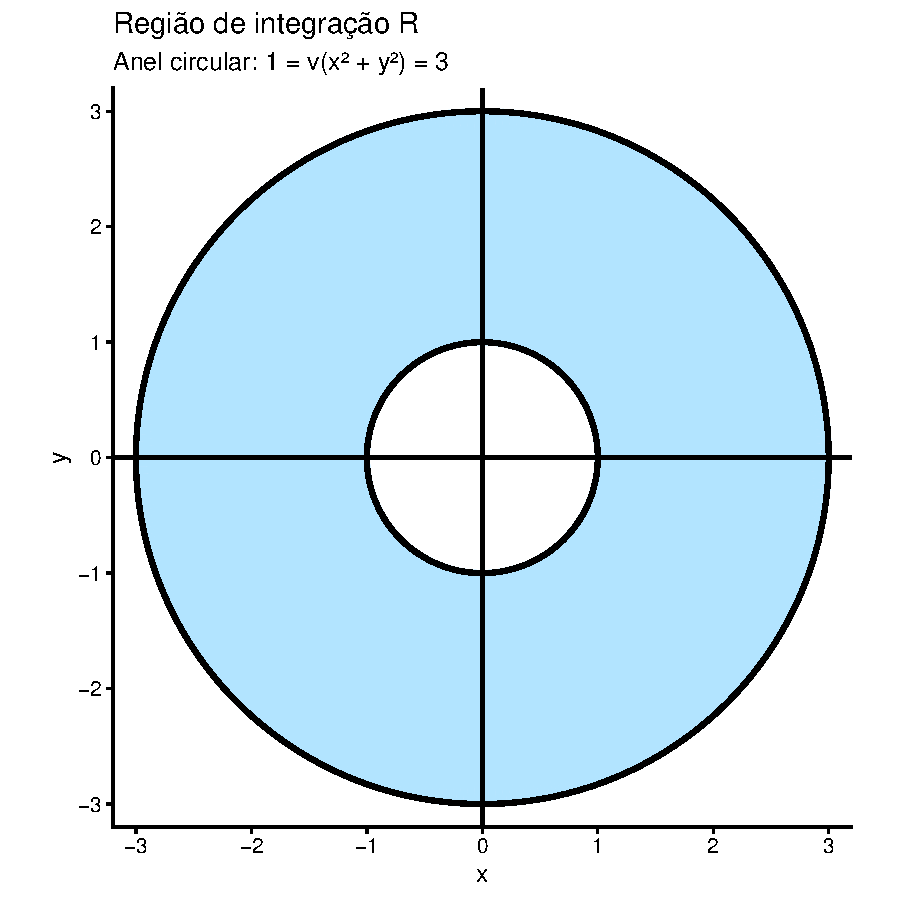
\includegraphics[keepaspectratio]{integrais_dup_trip_files/figure-beamer/unnamed-chunk-8-1.pdf}}
\end{center}
\end{frame}

\begin{frame}{Integral Dupla em Coordenadas Polares}
\phantomsection\label{integral-dupla-em-coordenadas-polares-8}
\textbf{Solução:} Em coordenadas polares:

\[
x=r\cos\theta,\qquad y=r\,\text{sen }\theta,\qquad dA=dx\,dy=r\,dr\,d\theta
\]

Além disso, \[
\sqrt{x^2+y^2}=\sqrt{r^2}=r \quad (r\ge 0)
\]

Como \(R\) é um anel completo, os limites são: \[
1\le r\le 3,\qquad 0\le \theta\le 2\pi
\]
\end{frame}

\begin{frame}{Integral Dupla em Coordenadas Polares}
\phantomsection\label{integral-dupla-em-coordenadas-polares-9}
Assim, \[
\iint_R \sqrt{x^2+y^2}\,dA
=
\int_{0}^{2\pi}\int_{1}^{3} r\cdot r\,dr\,d\theta
=
\int_{0}^{2\pi}\int_{1}^{3} r^2\,dr\,d\theta
\]

\begin{block}{Integral em \(r\)}
\phantomsection\label{integral-em-r}
\[
\int_{1}^{3} r^2\,dr
=
\left.\frac{r^3}{3}\right|_{1}^{3}
=
\frac{27-1}{3}
=
\frac{26}{3}
\]
\end{block}

\begin{block}{Integral em \(\theta\)}
\phantomsection\label{integral-em-theta}
\[
\int_{0}^{2\pi} \frac{26}{3} d\theta = \frac{26}{3} \int_{0}^{2\pi} d\theta = \frac{26}{3} \cdot \theta \bigg|_0^{2\pi} = \frac{52 \pi}{3}
\]
\end{block}
\end{frame}




\end{document}
